\documentclass[border=3pt,tikz]{standalone}
\usepackage{amsmath}
\usetikzlibrary{calc}
\usetikzlibrary{arrows.meta} % for arrow size
\begin{document}
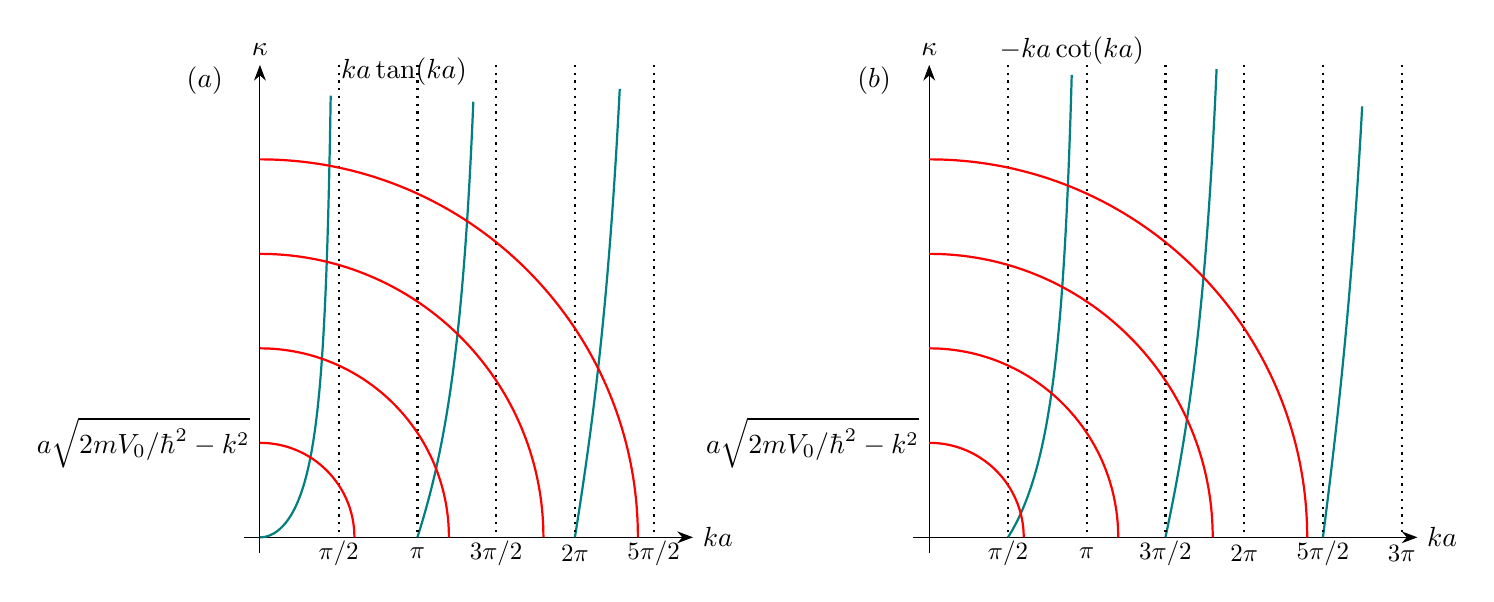
\begin{tikzpicture}[scale=1]

    
    \node [] at (-0.7, 5.8) {$(a)$};
    \draw[, -{Stealth[length=2mm]}] (0, -0.2) -- (0, 6) node [above] {$\kappa$} ;
    \draw[, -{Stealth[length=2mm]}] (-0.2, 0) -- (5.5, 0) node [right] {$ka$};
    \draw[teal, thick] plot[variable=\t, domain=0:0.9, samples=100, smooth,thick] ({\t}, {\t * tan( 90*\t)}) node [black, above right] {$ka \tan (ka)$};
    \draw[teal, thick] plot[variable=\t, domain=2:2.71, samples=100, smooth,thick] ({\t}, {\t * tan( 90*\t)});
    \draw[teal, thick] plot[variable=\t, domain=4:4.57, samples=100, smooth,thick] ({\t}, {\t * tan( 90*\t)}) ;
    
    \draw[thick, dotted] (1, 6) -- (1, 0);
    \node [scale=0.9] at (1, -0.2) {$\pi/2$};
    \draw[thick, dotted] (2, 6) -- (2, 0);
    \node [scale=0.9] at (2, -0.2) {$\pi$};
    \draw[thick, dotted] (3, 6) -- (3, 0);
    \node [scale=0.9] at (3, -0.2) {$3\pi/2$};
    \draw[thick, dotted] (4, 6) -- (4, 0);
    \node [scale=0.9] at (4, -0.2) {$2\pi$};
    \draw[thick, dotted] (5, 6) -- (5, 0);
    \node [scale=0.9] at (5, -0.2) {$5\pi/2$};
    
    \draw[red, thick] (1.2, 0) arc (0:90:1.2) node [black, left] {$a\sqrt{2mV_0/\hbar^2 - k^2}$};
    \draw[red, thick] (2.4, 0) arc (0:90:2.4);
    \draw[red, thick] (3.6, 0) arc (0:90:3.6);
    \draw[red, thick] (4.8, 0) arc (0:90:4.8);
    
    
    
    \begin{scope}[shift={(8.5,0)}]
    \node [] at (-0.7, 5.8) {$(b)$};
    \draw[, -{Stealth[length=2mm]}] (0, -0.2) -- (0, 6) node [above] {$\kappa$} ;
    \draw[, -{Stealth[length=2mm]}] (-0.2, 0) -- (6.2, 0) node [right] {$ka$};
    \draw[teal, thick] plot[variable=\t, domain=1:1.81, samples=100, smooth,thick] ({\t}, {-\t * cot( 90*\t)}) node[black, above] {$-ka \cot (ka)$};
    \draw[teal, thick] plot[variable=\t, domain=3:3.65, samples=100, smooth,thick] ({\t}, {-\t * cot( 90*\t)});
    \draw[teal, thick] plot[variable=\t, domain=5:5.5, samples=100, smooth,thick] ({\t}, {-\t * cot( 90*\t)});
    
    \draw[thick, dotted] (1, 6) -- (1, 0);
    \node [scale=0.9] at (1, -0.2) {$\pi/2$};
    \draw[thick, dotted] (2, 6) -- (2, 0);
    \node [scale=0.9] at (2, -0.2) {$\pi$};
    \draw[thick, dotted] (3, 6) -- (3, 0);
    \node [scale=0.9] at (3, -0.2) {$3\pi/2$};
    \draw[thick, dotted] (4, 6) -- (4, 0);
    \node [scale=0.9] at (4, -0.2) {$2\pi$};
    \draw[thick, dotted] (5, 6) -- (5, 0);
    \node [scale=0.9] at (5, -0.2) {$5\pi/2$};
    \draw[thick, dotted] (6, 6) -- (6, 0);
    \node [scale=0.9] at (6, -0.2) {$3\pi$};
    
    \draw[red, thick] (1.2, 0) arc (0:90:1.2) node[black, left] {$a\sqrt{2mV_0/\hbar^2-k^2}$};
    \draw[red, thick] (2.4, 0) arc (0:90:2.4);
    \draw[red, thick] (3.6, 0) arc (0:90:3.6);
    \draw[red, thick] (4.8, 0) arc (0:90:4.8);
    \end{scope}
    \end{tikzpicture}
\end{document}